\documentclass[aspectratio=169]{beamer}
\usepackage{booktabs}
\usepackage{graphicx}
\usepackage{adjustbox}
% \documentclass[aspectratio=43]{beamer}

% Define `accent`/`accent2` colors for theme customization
\definecolor{accent}{HTML}{006896}
\definecolor{accent2}{HTML}{E64173}

% Beamer theme
% Define colors ----------------------------------------------------------------
\usepackage{xcolor}

\definecolor{purple}{HTML}{695693}
\definecolor{cranberry}{HTML}{E64173}
\definecolor{orange}{HTML}{D65616}
\definecolor{navy}{HTML}{006896}
\definecolor{teal}{HTML}{1A505A}
\definecolor{ruby}{HTML}{9a2515}
\definecolor{alice}{HTML}{107895}
\definecolor{daisy}{HTML}{EBC944}
\definecolor{coral}{HTML}{F26D21}
\definecolor{kelly}{HTML}{829356}
\definecolor{slate900}{HTML}{131516}
\definecolor{asher}{HTML}{555F61}
\definecolor{slate}{HTML}{314F4F}

% Slate from Tailwind Colors
\definecolor{slate50}{HTML}{f8fafc}
\definecolor{slate100}{HTML}{f1f5f9}
\definecolor{slate200}{HTML}{e2e8f0}
\definecolor{slate300}{HTML}{cbd5e1}
\definecolor{slate400}{HTML}{94a3b8}
\definecolor{slate500}{HTML}{64748b}
\definecolor{slate600}{HTML}{475569}
\definecolor{slate700}{HTML}{334155}
\definecolor{slate800}{HTML}{1e293b}
\definecolor{slate900}{HTML}{0f172a}
\definecolor{slate950}{HTML}{020617}

% Easily color text
\newcommand\purple[1]{{\color{purple}#1}}
\newcommand\cranberry[1]{{\color{cranberry}#1}}
\newcommand\orange[1]{{\color{orange}#1}}
\newcommand\navy[1]{{\color{navy}#1}}
\newcommand\teal[1]{{\color{teal}#1}}
\newcommand\kelly[1]{{\color{kelly}#1}}
\newcommand\ruby[1]{{\color{ruby}#1}}
\newcommand\alice[1]{{\color{alice}#1}}
\newcommand\daisy[1]{{\color{daisy}#1}}
\newcommand\coral[1]{{\color{coral}#1}}

% Color background of text
\newcommand\bgNavy[1]{{\colorbox{navy!80!white}{#1}}}
\newcommand\bgOrange[1]{{\colorbox{orange!80!white}{#1}}}
\newcommand\bgTeal[1]{{\colorbox{teal!80!white}{#1}}}
\newcommand\bgPurple[1]{{\colorbox{purple!80!white}{#1}}}
\newcommand\bgKelly[1]{{\colorbox{kelly!80!white}{#1}}}
\newcommand\bgRuby[1]{{\colorbox{ruby!80!white}{#1}}}
\newcommand\bgAlice[1]{{\colorbox{alice!80!white}{#1}}}
\newcommand\bgDaisy[1]{{\colorbox{daisy!80!white}{#1}}}
\newcommand\bgCoral[1]{{\colorbox{coral!80!white}{#1}}}
\newcommand\bgCranberry[1]{{\colorbox{cranberry!80!white}{#1}}}

% Beamer Options ---------------------------------------------------------------

% Background
\setbeamercolor{background canvas}{bg = white}

% Change text margins
\setbeamersize{text margin left = 15pt, text margin right = 15pt} 

% \alert
\setbeamercolor{alerted text}{fg = accent2}

% Frame title
\setbeamercolor{frametitle}{bg = white, fg = slate900}
\setbeamercolor{framesubtitle}{bg = white, fg = accent}
\setbeamerfont{framesubtitle}{size = \small, shape = \itshape}

% Page numbering
\usepackage{appendixnumberbeamer}
\setbeamercolor{page number in head/foot}{fg=slate600}
\setbeamertemplate{footline}[frame number]

% Table of Contents
\setbeamercolor{section in toc}{fg = slate700}
\setbeamercolor{subsection in toc}{fg = slate900}

% Button 
\setbeamercolor{button}{bg = white, fg = slate900}
\setbeamerfont{button}{}
\setbeamercolor{button border}{fg = accent}

% Remove navigation symbols
\setbeamertemplate{navigation symbols}{}

% Table and Figure captions
\setbeamercolor{caption}{fg = slate900!70!white}
\setbeamercolor{caption name}{fg=slate900}
\setbeamerfont{caption name}{shape = \itshape}

% Links
\usepackage{hyperref}
\hypersetup{
  colorlinks = true,
  linkcolor = accent2,
  filecolor = accent2,
  urlcolor = accent2,
  citecolor = accent2,
}

% Line spacing
\usepackage{setspace}
\setstretch{1.3}

% Remove annoying over-full box warnings
\vfuzz2pt 
\hfuzz2pt


% Title page -------------------------------------------------------------------
\setbeamercolor{title}{fg = slate900}
\setbeamercolor{subtitle}{fg = accent}

%% Custom \maketitle and \titlepage
\setbeamertemplate{title page}
{
  %\begin{centering}
  \vspace{20mm}
  {\Large \usebeamerfont{title}\usebeamercolor[fg]{title}\inserttitle}\\ \vskip0.25em%
  \ifx\insertsubtitle\@empty%
  \else%
    {\usebeamerfont{subtitle}\usebeamercolor[fg]{subtitle}\insertsubtitle\par}%
  \fi% 
  {\vspace{10mm}\insertauthor}\\
  {\color{asher}\small{\insertdate}}\\
  %\end{centering}
}

% Table of Contents with Sections ----------------------------------------------
\setbeamerfont{myTOC}{series=\bfseries, size=\Large}
\AtBeginSection[]{
  \begin{frame}{Roadmap}
    \tableofcontents[current]   
  \end{frame}
}

% Block ------------------------------------------------------------------------
\usepackage{tcolorbox}

\defbeamertemplate{block begin}{framed}[1][] {
  \begin{tcolorbox}[colback=slate50, colframe=slate200, arc=0mm]
  {
    \vskip\smallskipamount%
    \ifthenelse{\equal{#1}{}}{}{%
      \raggedright\usebeamerfont*{block title}\usebeamercolor[fg]{title}%
      \textbf{\insertblocktitle}%
      \vskip\medskipamount%
    }
  }%
  \raggedright%
  \usebeamerfont{block body}%
}
\defbeamertemplate{block end}{framed}[1][] {
  \vskip\smallskipamount\end{tcolorbox}
}
\setbeamertemplate{blocks}[framed]

% Colors from plugging base color into https://uicolors.app/create
\usepackage{ifthen}
\newenvironment*{slateBlock}[1]{%
  \begin{tcolorbox}[colback=slate50, colframe=slate200, arc=0mm]{
    \vskip\smallskipamount%
    \ifthenelse{\equal{#1}{}}{}{%
      \raggedright\usebeamerfont*{block title}\usebeamercolor[fg]{title}%
      \textbf{#1}%
      \vskip\medskipamount%
    }%
  }%
  \raggedright%
  \usebeamerfont{block body}%
}{%
  \vskip\smallskipamount\end{tcolorbox}
}

\definecolor{purple50}{HTML}{f9f8fc}
\definecolor{purple100}{HTML}{f1eff8}
\definecolor{purple200}{HTML}{e6e2f2}
\newenvironment*{purpleBlock}[1]{%
  \begin{tcolorbox}[colback=purple50, colframe=purple200, arc=0mm]{
    \vskip\smallskipamount%
    \ifthenelse{\equal{#1}{}}{}{%
      \raggedright\usebeamerfont*{block title}\usebeamercolor[fg]{title}%
      \textbf{#1}%
      \vskip\medskipamount%
    }%
  }%
  \raggedright%
  \usebeamerfont{block body}%
}{%
  \vskip\smallskipamount\end{tcolorbox}
}

\definecolor{cranberry50}{HTML}{fdf2f6}
\definecolor{cranberry100}{HTML}{fbe8ef}
\definecolor{cranberry200}{HTML}{fad0e0}
\newenvironment*{cranberryBlock}[1]{%
  \begin{tcolorbox}[colback=cranberry50, colframe=cranberry200, arc=0mm]{
    \vskip\smallskipamount%
    \raggedright\usebeamerfont*{block title}\usebeamercolor[fg]{title}%
    \textbf{#1}%
  }%
  \vskip\medskipamount%
  \raggedright%
  \usebeamerfont{block body}%
}{%
  \vskip\smallskipamount\end{tcolorbox}
}

% Bullet points ----------------------------------------------------------------

%% Fix left-margins
\settowidth{\leftmargini}{\usebeamertemplate{itemize item}}
\addtolength{\leftmargini}{\labelsep}

%% enumerate item color
\setbeamercolor{enumerate item}{fg = slate600}
\setbeamerfont{enumerate item}{size = \small}
\setbeamertemplate{enumerate item}{\insertenumlabel.}

%% itemize
\setbeamercolor{itemize item}{fg = slate600}
\setbeamerfont{itemize item}{size = \small}
\setbeamertemplate{itemize item}[circle]

%% right arrow for subitems
\setbeamercolor{itemize subitem}{fg = slate600}
\setbeamerfont{itemize subitem}{size = \small}
\setbeamertemplate{itemize subitem}{$\rightarrow$}

\setbeamercolor{itemize subsubitem}{fg = slate600}
\setbeamerfont{itemize subsubitem}{size = \small}
\setbeamertemplate{itemize subsubitem}[square]

% References -------------------------------------------------------------------

%% Bibliography Font, roughly matching aea
\setbeamerfont{bibliography item}{size = \footnotesize}
\setbeamerfont{bibliography entry author}{size = \footnotesize, series = \bfseries}
\setbeamerfont{bibliography entry title}{size = \footnotesize}
\setbeamerfont{bibliography entry location}{size = \footnotesize, shape = \itshape}
\setbeamerfont{bibliography entry note}{size = \footnotesize}

\setbeamercolor{bibliography item}{fg = slate900}
\setbeamercolor{bibliography entry author}{fg = accent!60!slate900}
\setbeamercolor{bibliography entry title}{fg = slate900}
\setbeamercolor{bibliography entry location}{fg = slate900}
\setbeamercolor{bibliography entry note}{fg = slate900}

%% Remove bibliography symbol in slides
\setbeamertemplate{bibliography item}{}


% \begin{columns} --------------------------------------------------------------
\usepackage{multicol}


% Fonts ------------------------------------------------------------------------
% Beamer Option to use custom fonts
\usefonttheme{professionalfonts}

% \usepackage[utopia, smallerops, varg]{newtxmath}
% \usepackage{utopia}
\usepackage[sfdefault,light]{roboto}

% Small adjustments to text kerning
\usepackage{microtype}

% For \underbracket/\overbracket
\usepackage{mathtools}

% References -------------------------------------------------------------------
\usepackage[
    citestyle= authoryear,
    style = authoryear,
    natbib = true, 
    backend = biber
]{biblatex}

% Smaller font-size for references
\renewcommand*{\bibfont}{\small}

% Remove "In:"
\renewbibmacro{in:}{}

% Color citations for slides 
\newenvironment{citecolor}
    {\footnotesize\begin{color}{accent2}}
    {\end{color}}

\newcommand{\citetcolor}[1]{{\footnotesize\textcolor{gray}{\citet{#1}}}}
\newcommand{\citepcolor}[1]{{\footnotesize\textcolor{gray}{\citep{#1}}}}

% Tables -----------------------------------------------------------------------

% When tables are too big, use adjustbox
% \begin{adjustbox}{width = 1.2\textwidth, center}
\usepackage{adjustbox}
\usepackage{array}
\usepackage{threeparttable, booktabs, adjustbox}
    
% Fix \input with tables
% \input fails when \\ is at end of external .tex file
\makeatletter
\let\input\@@input
\makeatother

% Tables too narrow
% \begin{tabularx}{\linewidth}{cols}
% col-types: X - center, L - left, R -right
% Relative scale: >{\hsize=.8\hsize}X/L/R
\usepackage{tabularx}
\newcolumntype{L}{>{\raggedright\arraybackslash}X}
\newcolumntype{R}{>{\raggedleft\arraybackslash}X}
\newcolumntype{C}{>{\centering\arraybackslash}X}

% Table Highlighting -----------------------------------------------------------
% Create top-left and bottom-right markets in tabular cells with a unique matching id and these commands will outline those cells
\usepackage[beamer,customcolors]{hf-tikz}
\usetikzlibrary{calc}
\usetikzlibrary{fit,shapes.misc}

% To set the hypothesis highlighting boxes red.
\newcommand\marktopleft[1]{%
    \tikz[overlay,remember picture] 
        \node (marker-#1-a) at (0,1.5ex) {};%
}
\newcommand\markbottomright[1]{%
    \tikz[overlay,remember picture] 
        \node (marker-#1-b) at (0,0) {};%
    \tikz[accent!80!slate900, ultra thick, overlay, remember picture, inner sep=4pt]
        \node[draw, rectangle, fit=(marker-#1-a.center) (marker-#1-b.center)] {};%
}

% Figures ----------------------------------------------------------------------

% \imageframe{img_name}
% from https://github.com/mattslate900well/cousteau
\newcommand{\imageframe}[1]{%
    \begin{frame}[plain]
        \begin{tikzpicture}[remember picture, overlay]
            \node[at = (current page.center), xshift = 0cm] (cover) {%
                \includegraphics[keepaspectratio, width=\paperwidth, height=\paperheight]{#1}
            };
        \end{tikzpicture}
    \end{frame}%
}

% subfigures
\usepackage{subfigure}

% Highlight slide --------------------------------------------------------------
% \begin{transitionframe} Text \end{transitionframe}
% from paulgp's beamer tips
\newenvironment{transitionframe}{
    \setbeamercolor{background canvas}{bg=accent!60!black}
    \begin{frame}\color{white}\LARGE\centering
}{
    \end{frame}
}



% Title --------------------------------------------
\title{CU Denver Math Camp - Limits \& Derivatives}
\subtitle{Day 2}
\date{August 6, 2024}
\author{Michael R. Karas}

\begin{document}

% ------------------------------------------------------------------------------
\begin{frame}
\maketitle

% \vspace{2.5mm}
{\footnotesize University of Colorado, Boulder}
\end{frame}
% ------------------------------------------------------------------------------

%------------------------------------------------------------------------------
\begin{frame}{Day 2 Topics}\label{main1}

\begin{itemize}
	\begin{itemize}
		\item Practice Problems		
		\item Increasing/Decreasing Functions
		\item Concave/Convex Functions
		\item Implicit Differentiation
		\item Partial Derivatives
		\item Taylor Series
	\end{itemize}
\end{itemize}
\end{frame}
%------------------------------------------------------------------------------

%------------------------------------------------------------------------------
\begin{frame}{Day 1 Practice Problems}\label{main1}
	\vspace{-4cm}
    \[
    f(x) = \frac{2x}{x^{2}+2}
    \]
\end{frame}
%------------------------------------------------------------------------------

%------------------------------------------------------------------------------
\begin{frame}{Day 1 Practice Problems}\label{main1}
	\vspace{-4cm}
    \[
    f(x) = e^{x^{2} + ln(x)}
    \]
\end{frame}
%------------------------------------------------------------------------------

%------------------------------------------------------------------------------
\begin{frame}{Day 1 Practice Problems}\label{main1}
	\vspace{-4cm}
    \[
    f(x) = x(x^{2} + 1)
    \]
    Find \( f'(x) \) and \( f''(x) \)
\end{frame}
%------------------------------------------------------------------------------

%------------------------------------------------------------------------------
\begin{frame}{Day 1 Practice Problems}\label{main1}
	\vspace{-4cm}
    \[
    f(x) = ln(x^{2} + 1)
    \]
    Find \( f'(x) \) and \( f''(x) \)
\end{frame}
%------------------------------------------------------------------------------

%------------------------------------------------------------------------------
\begin{frame}{Day 1 Practice Problems}\label{main1}
	\vspace{-4cm}
    Prove that \( \frac{d}{dx}e^{x} = e^{x} \)
\end{frame}
%------------------------------------------------------------------------------

%------------------------------------------------------------------------------
\begin{frame}{Increasing/Decreasing Functions}\label{main1}
    Let $f$ be a differentiable function defined on an interval $[a, b]$
    \begin{itemize}
        \item $f$ is increasing on $[a, b]$ if, for every $a \leq x \leq b$, $f'(x) > 0$
        \item $f$ is decreasing on $[a, b]$ if, for every $a \leq x \leq b$, $f'(x) \leq 0$
    \end{itemize}
    Could replace $\leq$ with $<$ and say “strictly increasing” (no flat parts of $f$ on $[a, b]$), likewise with decreasing. When $f'(x) = 0$ the function is not changing, an “optimal” point.

\end{frame}
%------------------------------------------------------------------------------

%------------------------------------------------------------------------------
\begin{frame}{Increasing/Decreasing Functions Practice Problems}\label{main1}
	\vspace{-4cm}
     \[
    f(x) = x^{2}
    \]
    Find which intervals which \( f(x) \) is increasing and which intervals which \( f(x) \) is decreasing.
\end{frame}
%------------------------------------------------------------------------------

%------------------------------------------------------------------------------
\begin{frame}{Increasing/Decreasing Functions Practice Problems}\label{main1}
	\vspace{-4cm}
     \[
    f(x) = ln(x)
    \]
    Find which intervals which \( f(x) \) is increasing and which intervals which \( f(x) \) is decreasing.
\end{frame}
%------------------------------------------------------------------------------

%------------------------------------------------------------------------------
\begin{frame}{Increasing/Decreasing Functions Practice Problems}\label{main1}
	\vspace{-4cm}
     \[
    f(x) = e^{x}
    \]
    Find which intervals which \( f(x) \) is increasing and which intervals which \( f(x) \) is decreasing.
\end{frame}
%------------------------------------------------------------------------------

%------------------------------------------------------------------------------
\begin{frame}{Concave/Convex Functions}\label{main1}
    Often it is not enough to know if a function is increasing/decreasing. We need to know its shape. Let $f$ and $I$ be as before. Then,
    \begin{itemize}
        \item $f$ is convex on $[a, b]$ if, for every $a \leq x \leq b$, $f''(x) > 0$
        \item $f$ is concave on $[a, b]$ if, for every $a \leq x \leq b$, $f''(x) < 0$
    \end{itemize}
    Convex: function is increasing at an increasing rate to the bottom of a “valley.” Concave: function is increasing at a decreasing rate to the peak of a “mountain.”
    \begin{itemize}
        \item If $f''(x) = 0$, $f$ is at an inflection point – the acceleration switches (e.g. skiing)
    \end{itemize}
\end{frame}
%------------------------------------------------------------------------------

%------------------------------------------------------------------------------
\begin{frame}{Concave/Convex Functions}\label{main1}
    \begin{figure}
        \centering
        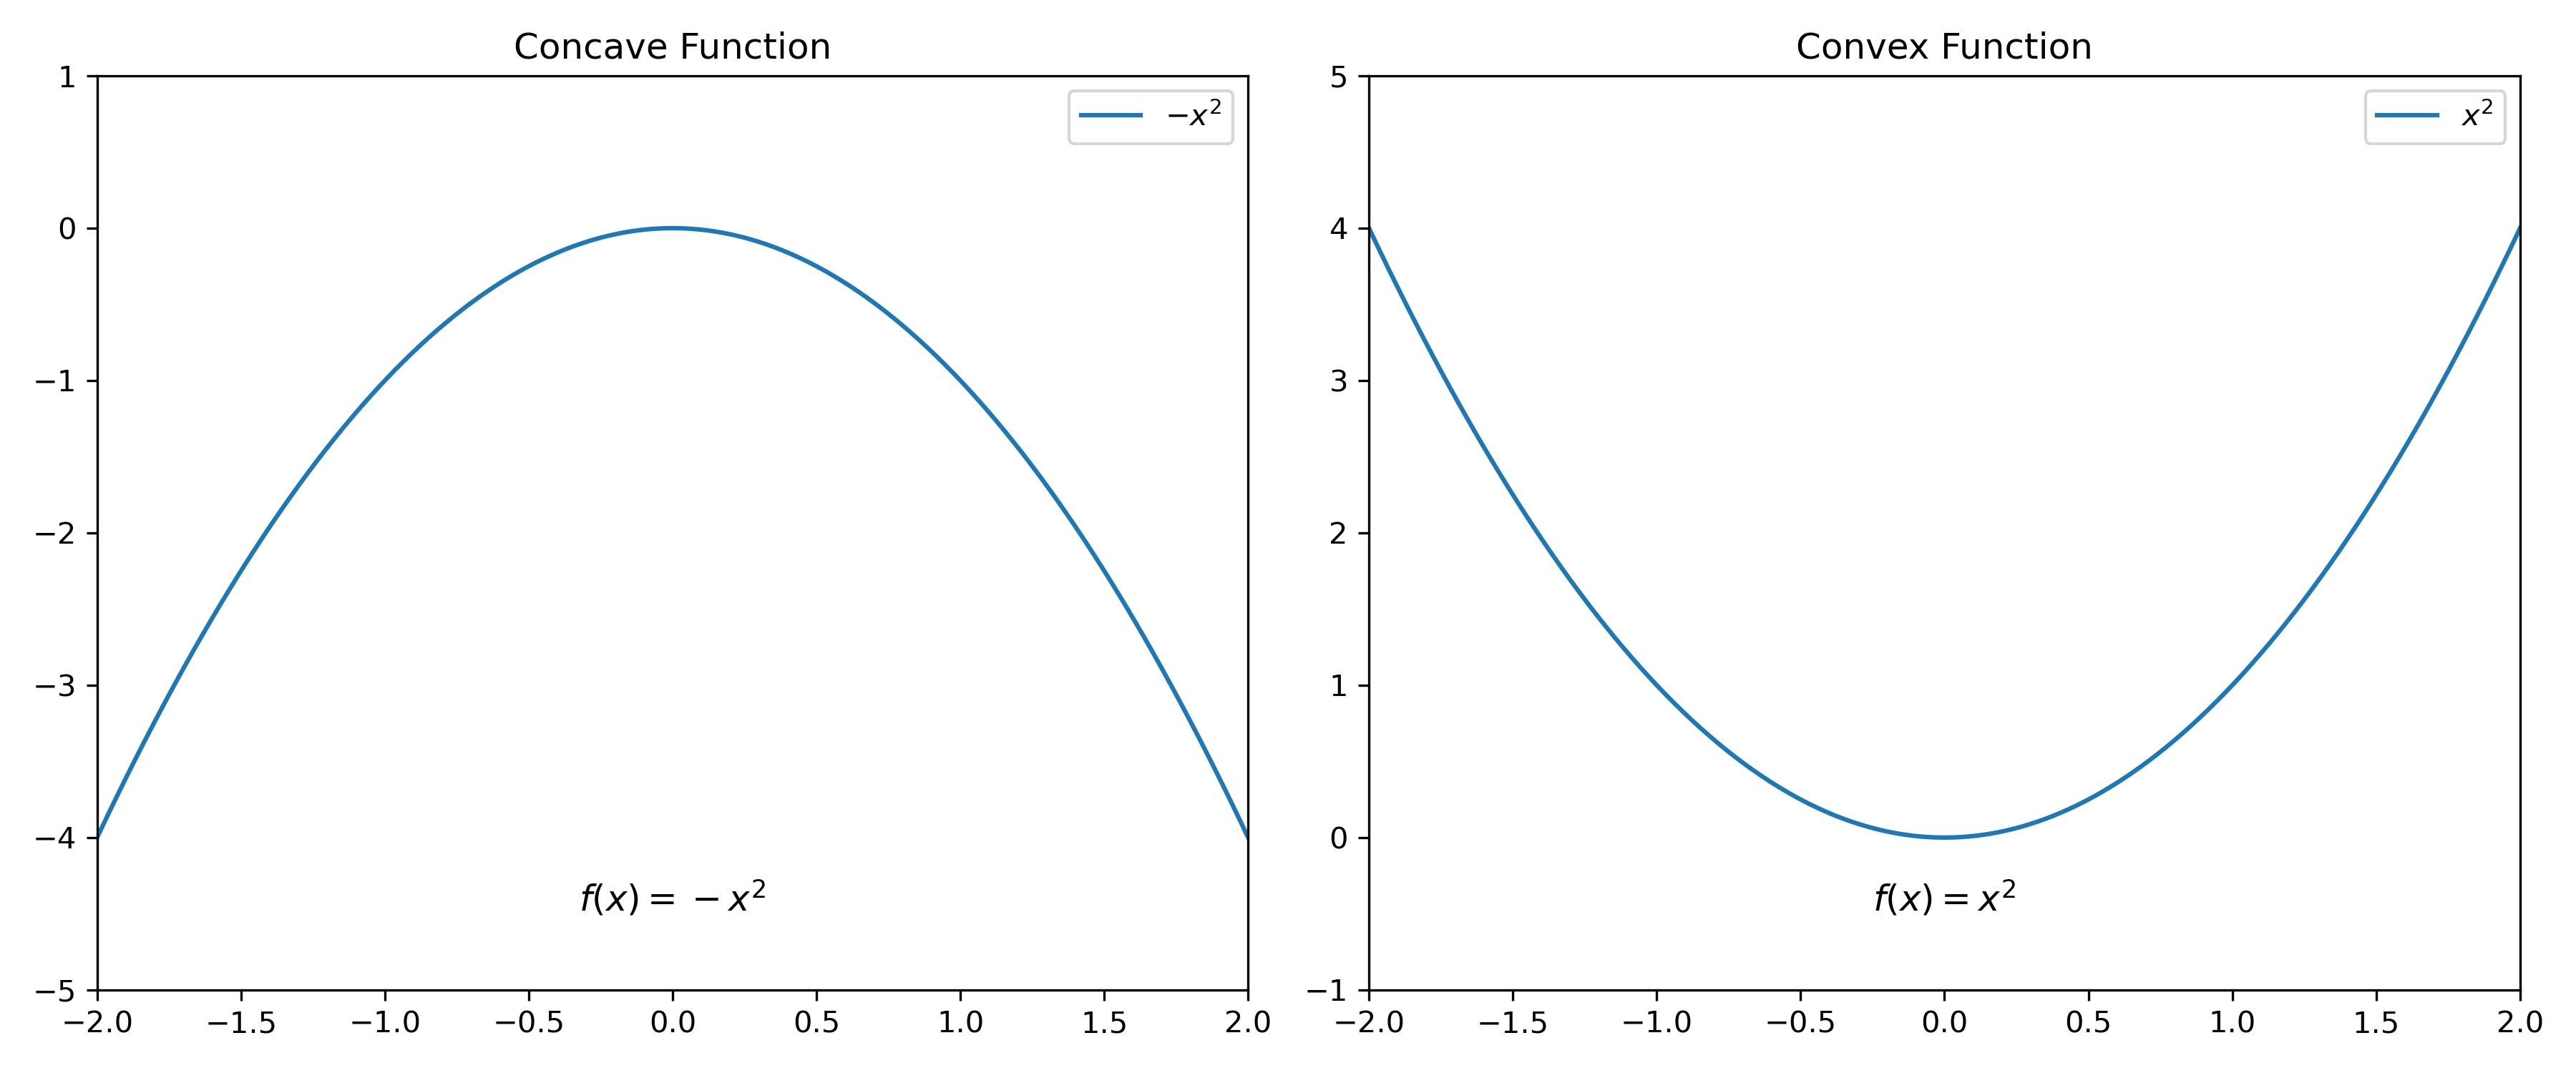
\includegraphics[width=0.9\textwidth]{/Users/michaelkaras/Documents/CU_Denver_Math_Camp/concave_convex_example.jpg}
    \end{figure}
\end{frame}
%------------------------------------------------------------------------------

%------------------------------------------------------------------------------
\begin{frame}{Concave/Convex Functions Practice Problems}\label{main1}
	\vspace{-4cm}
     \[
    f(x) = x - 2ln(x+1)
    \]
\end{frame}
%------------------------------------------------------------------------------

%------------------------------------------------------------------------------
\begin{frame}{Implicit Differentiation}\label{main1}
    Sometimes we can’t solve for $y = f(x)$ (or it would be very difficult) but still need to differentiate. Implicit differentiation allows us to find $f'(x)$ without a “closed-form” solution for $y = f(x)$.
    \begin{itemize}
    \begin{itemize}
        \item Differentiate both sides of the equation using all the typical rules of derivatives, treating $x$ and $y$ as variables that are both changing
        \item If you differentiate something involving $y$, multiply the answer by $y'$ (the derivative of $y = f(x)$)
        \item If you differentiate something involving $x$, do not multiply by anything new
        \item After everything is differentiated, solve for $y'$ using algebra
        \item The answer for $y'$ should be a function of $x$ (and potentially $y$)
    \end{itemize}
    \end{itemize}
\end{frame}
%------------------------------------------------------------------------------

%------------------------------------------------------------------------------
\begin{frame}{Implicit Differentiation}\label{main1}
    Suppose $x + y + xy = 5$.
    \[
    1 + 1 \cdot y' + \underbrace{1 \cdot y}_{f'(x)g(x)} + \underbrace{x \cdot 1 \cdot y'}_{f(x)g'(x)} = 0
    \]
    Using product rule:
    \[
    1 + y' + y + xy' = 0
    \]
    \[
    y'(1 + x) = -1 - y
    \]
    \[
    y' = \frac{-1 - y}{1 + x}
    \]
    The derivative is a function of both $x$ and $y$.
\end{frame}
%------------------------------------------------------------------------------

%------------------------------------------------------------------------------
\begin{frame}{Implicit Differentiation Practice Problems}\label{main1}
	\vspace{-4cm}
     \[
    x^{2} + y^{2} = 1
    \]
\end{frame}
%------------------------------------------------------------------------------

%------------------------------------------------------------------------------
\begin{frame}{Partial Derivatives}\label{main1}
    The function $z = f(x, y)$ takes two inputs and outputs a third.  We can evaluate what happens to that output when we change $x$ or $y$ (but not both).
    \begin{itemize}
        \item $\frac{\partial z}{\partial x} =$ “the derivative of $z$ with respect to $x$”
        \begin{itemize}
        \item The slope of $f$ in the cardinal direction of $x$ (e.g. “north-south”)
        \item The tangent of $f$ in the $x$ direction at a point $(x_0, y_0)$
        \end{itemize}
        \item $\frac{\partial z}{\partial y} =$ “the derivative of $z$ with respect to $y$”
        \begin{itemize}
        \item The slope of $f$ in the cardinal direction of $y$ (e.g. “east-west”)
        \item The tangent of $f$ in the $y$ direction at a point $(x_0, y_0)$
    	\end{itemize}
    \end{itemize}
\end{frame}
%------------------------------------------------------------------------------

%------------------------------------------------------------------------------
\begin{frame}{Partial Derivatives}\label{main1}
    All of these mean “take the partial derivative of $f$ with respect to $x$”:
    \begin{itemize}
        \item $f_x(x, y)$
        \item $\frac{\partial f(x, y)}{\partial x}$
        \item $\frac{\partial}{\partial x} f(x, y)$
        \item $\frac{\partial z}{\partial x}$ if $z = f(x, y)$
    \end{itemize}
\end{frame}
%------------------------------------------------------------------------------

%------------------------------------------------------------------------------
\begin{frame}{Partial Derivatives}\label{main1}
    Interpret $\frac{\partial z}{\partial x}$ as “what happens to $z$ if I change $x$, holding $y$ constant.” Likewise for $\frac{\partial z}{\partial y}$.
 	Suppose $z = x + y + xy$, find $\frac{\partial z}{\partial x}$.
    \[
    \frac{\partial z}{\partial x} = \frac{\partial}{\partial x} [x + y + xy] = \frac{\partial}{\partial x} x + \frac{\partial}{\partial x} y + \frac{\partial}{\partial x} xy = 1 + 0 + y \cdot 1 = 1 + y
    \]
\end{frame}
%------------------------------------------------------------------------------

%------------------------------------------------------------------------------
\begin{frame}{Partial Derivatives}\label{main1}
    The first partial derivatives $f_x(x, y)$ and $f_y(x, y)$ are themselves functions of $x$ and $y$. We could differentiate each of them with respect to either $x$ or $y$, so there are four second-order partial derivatives.
    \[
    f(x, y)
    \]
    \[
    \frac{\partial f}{\partial x} \quad \frac{\partial f}{\partial y}
    \]
    \[
    \frac{\partial^2 f}{\partial x^2} \quad \frac{\partial^2 f}{\partial y \partial x} \quad \frac{\partial^2 f}{\partial x \partial y} \quad \frac{\partial^2 f}{\partial y^2}
    \]

\end{frame}
%------------------------------------------------------------------------------

%------------------------------------------------------------------------------
\begin{frame}{Partial Derivatives}\label{main1}
    All of these mean “take the partial derivative of $f$ with respect to $x$ twice”:
    \begin{itemize}
        \item $f_{xx}(x, y)$
        \item $\frac{\partial^2 f(x, y)}{\partial x^2}$
        \item $\frac{\partial^2}{\partial x^2} f(x, y)$
        \item $\frac{\partial^2 z}{\partial x^2}$ if $z = f(x, y)$
    \end{itemize}
\end{frame}
%------------------------------------------------------------------------------

%------------------------------------------------------------------------------
\begin{frame}{Partial Derivatives}\label{main1}
    All of these mean “take the partial derivative of $f$ with respect to $x$, then with respect to $y$”:
    \begin{itemize}
        \item $f_{xy}(x, y)$
        \item $\frac{\partial^2 f(x, y)}{\partial y \partial x}$
        \item $\frac{\partial^2}{\partial y \partial x} f(x, y)$
        \item $\frac{\partial^2 z}{\partial y \partial x}$ if $z = f(x, y)$
    \end{itemize}
\end{frame}
%------------------------------------------------------------------------------

%------------------------------------------------------------------------------
\begin{frame}{Young's Theorem}\label{main1}
    If $f(x, y)$ is a twice differentiable function and continuous at the point $(x_0, y_0)$, then
    \[
    f_{xy}(x_0, y_0) = f_{yx}(x_0, y_0)
    \]
    The cross-partial derivatives are the same, regardless of the order in which you take them.
\end{frame}
%------------------------------------------------------------------------------

%------------------------------------------------------------------------------
\begin{frame}{Partial Derivatives Practice Problems}\label{main1}
	\vspace{-4cm}
     \[
    f(x,y) = x^{2} + y^{2} + x^{2}y^{2}
    \]
\end{frame}
%------------------------------------------------------------------------------

%------------------------------------------------------------------------------
\begin{frame}{Partial Derivatives Practice Problems}\label{main1}
	\vspace{-4cm}
     \[
    f(x,y) = x^{2}y+ln(x)y^{3}
    \]
\end{frame}
%------------------------------------------------------------------------------

%------------------------------------------------------------------------------
\begin{frame}{Taylor Series}\label{main1}
Sometimes it is too difficult (or not possible) to differentiate a function.  We can use a Taylor Series expansion to approximate the value of a function around different points.

For a function $f(x)$ with derivatives of all orders at $x=a$, the Taylor series is:
\[
f(x) = \sum_{n=0}^{\infty} \frac{f^{(n)}(a)}{n!} (x - a)^n
\]
When $a=0$, it is called the Maclaurin series.

\end{frame}
%------------------------------------------------------------------------------

%------------------------------------------------------------------------------
\begin{frame}{Taylor Series}\label{main1}
Taylor Series for $f(x) = \frac{1}{x}$
\[
f(x) = \frac{1}{x} \quad f'(x) = -\frac{1}{x^2} \quad f''(x) = \frac{2}{x^3} \quad f^{(k)}(x) = \frac{k!}{x^{k+1}}
\]
\[
P_k(x) = f(a) + f'(a)(x - a) + \frac{f''(a)}{2!}(x - a)^2 + \ldots + \frac{f^{(k)}(a)}{k!}(x - a)^k
\]
At $a=1$ of order $k==2$:
\[
P_2(x) = 1 - (x - 1) + (x - 1)^2
\]
At $a=3$ of order $k=2$:
\[
P_3(x) = \frac{1}{3} - \frac{x - 3}{3^2} + \frac{(x - 3)^2}{3^3}
\]

\end{frame}
%------------------------------------------------------------------------------

%------------------------------------------------------------------------------
\begin{frame}{Taylor Series}\label{main1}
    \begin{figure}
        \centering
        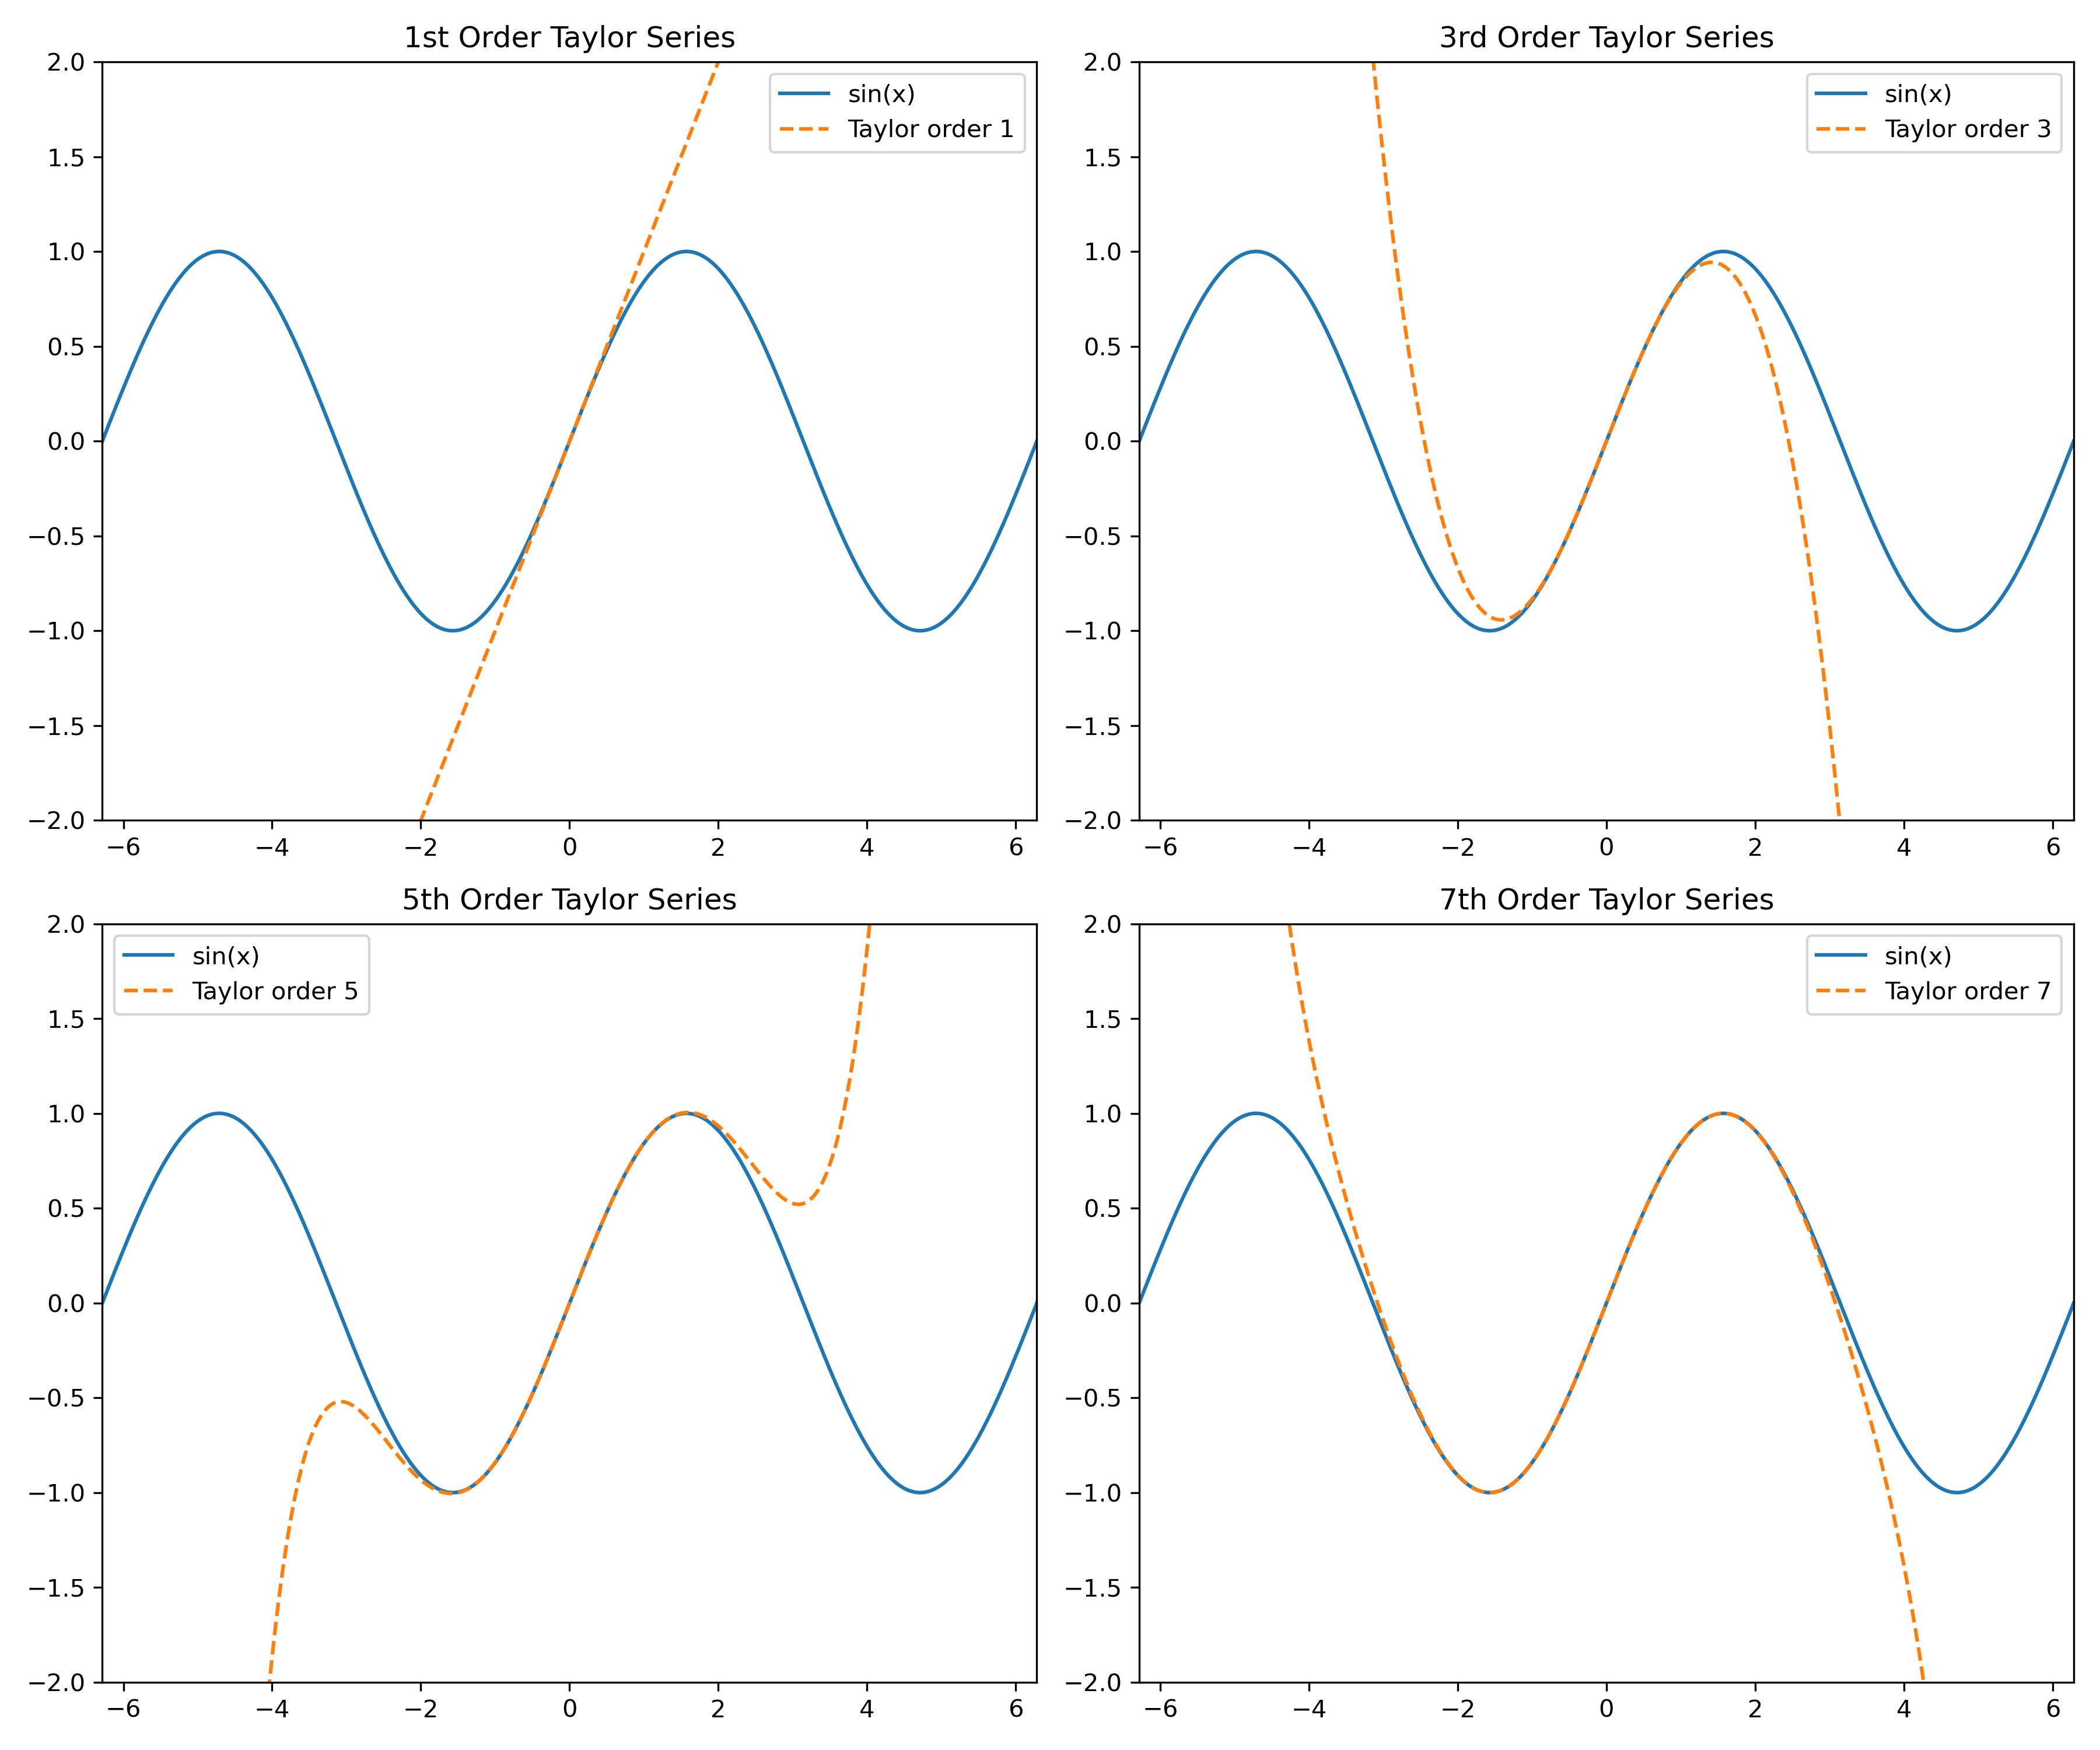
\includegraphics[width=0.6\textwidth]{/Users/michaelkaras/Documents/CU_Denver_Math_Camp/taylor_series_example.jpg}
    \end{figure}
\end{frame}
%------------------------------------------------------------------------------

%------------------------------------------------------------------------------
\begin{frame}{Taylor Series Practice Problems}\label{main1}
	\vspace{-4cm}
Write the Taylor Series Expansion of order k generated for the function \( f(x) = e^{x} \) around the point \( x = 0 \)
\end{frame}
%------------------------------------------------------------------------------



\end{document}
